 \chapter{Методика исследования}

 \section{Использование информации о фактическом времени ответа}

Выражение для прогнозного времени ответа можно использовать для выявления абер\-раций (отклонений) в поведении пользователя. Для этого введём понятие отклонения прогноза.

Отклонением прогноза будем разность между прогнозным временем ответа и фактичес\-ким временем ответа студента. В логарифмической шкале разность будет иметь вид отноше\-ния
\begin{equation}
E_{ij} = \ln \tilde{T}_{ij} - \ln t_{ij} =  \ln \frac{\tilde{T}_{ij}}{t_{ij}}
\end{equation}

Из этого отношения можно сделать вывод, что ошибка прогноза - случайная величина, которая имеет нормальное распределение c параметрами
\begin{equation}
E_{ij} \sim N\left(\mu + \beta_i + \tau_j - \ln t_{ij},\frac{n\sigma^2}{n-1}\right).
\end{equation}

Таким образом, выявление отклонений в поведении студента сводится к задаче проверки статистической гипотезы о том, что реализации $e_{ij}$ случайной величины $E_{ij}$ имеют нормаль\-ное распределение против альтернативы, что ошибка прогноза имеет какое-либо другое распреде\-ление
$$
\begin{array}{lll}
H_0 &:& e_{ij} \sim N\left(\mu + \beta_i + \tau_j - \ln t_{ij},\frac{n\sigma^2}{n-1}\right)\\
H_1 &:& \mbox{ошибка прогноза имеет другое распределение}
\end{array}
$$

\section{Обработка экспериментальных данных}

\subsection{Источник экспериментальных данных}

Для применения на практике теоретических положений и математических моделей, описанных в Главе \ref{ch22} использовались реальные данные пользователей системы дистанцион\-ного обучения МАИ. На момент написания диплома в системе не фиксировалось время, которое студент тратит на решение контрольных и тестовых задач. В связи с этим в исходный код системы дистанционного обучения и структуру базы данных, которая исполь\-зуется системой дистанционного обучения, были внесены доработки, позволяющие фикси\-ровать время ответа для всех существующих курсов (<<Математический анализ>>, <<Линейная алгебра и аналитическая геометрия>>, <<Теория вероятностей и математическая статистика>>).

После внесённых изменений система фиксирует следующие данные: сколько раз была отображена каждая задача, сколько попыток произвел каждый студент для её решения, какое количество времени было затрачено для каждой из попыток и насколько удачной была попытка (верно или неверно решена задача)

\subsection{Обработка полученных данных}

Для получения оценок параметров модели, описанных в разделе \ref{opm}, обработаем полученную статистику. Порядок обработки статистики покажем на примере задачи № 8.2.3 из курса <<Математический анализ>>

Вначале построим гистограмму для времени, которое студенты затрачивали для ответа на задачу
\begin{figure}[ht!]
\centering 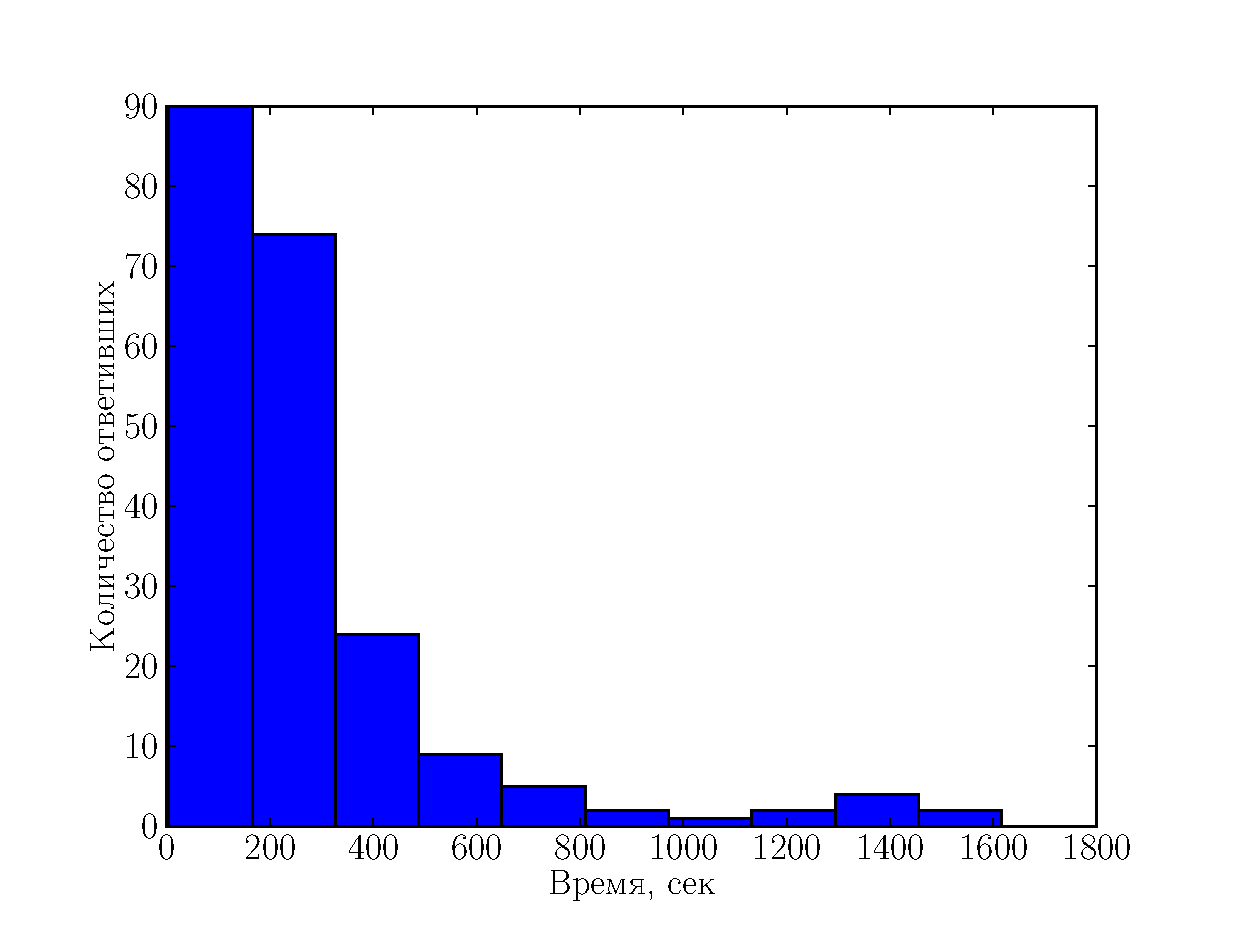
\includegraphics[scale=0.6]{test.eps}
\caption{Гистограмма времени ответа}
\end{figure}

Согласно модели, построенной в разделе \ref{mvonu}, применим логарифмическое \\преобразование к времени ответа и построим гистограмму полученных значений:
\begin{figure}[ht!]
\centering 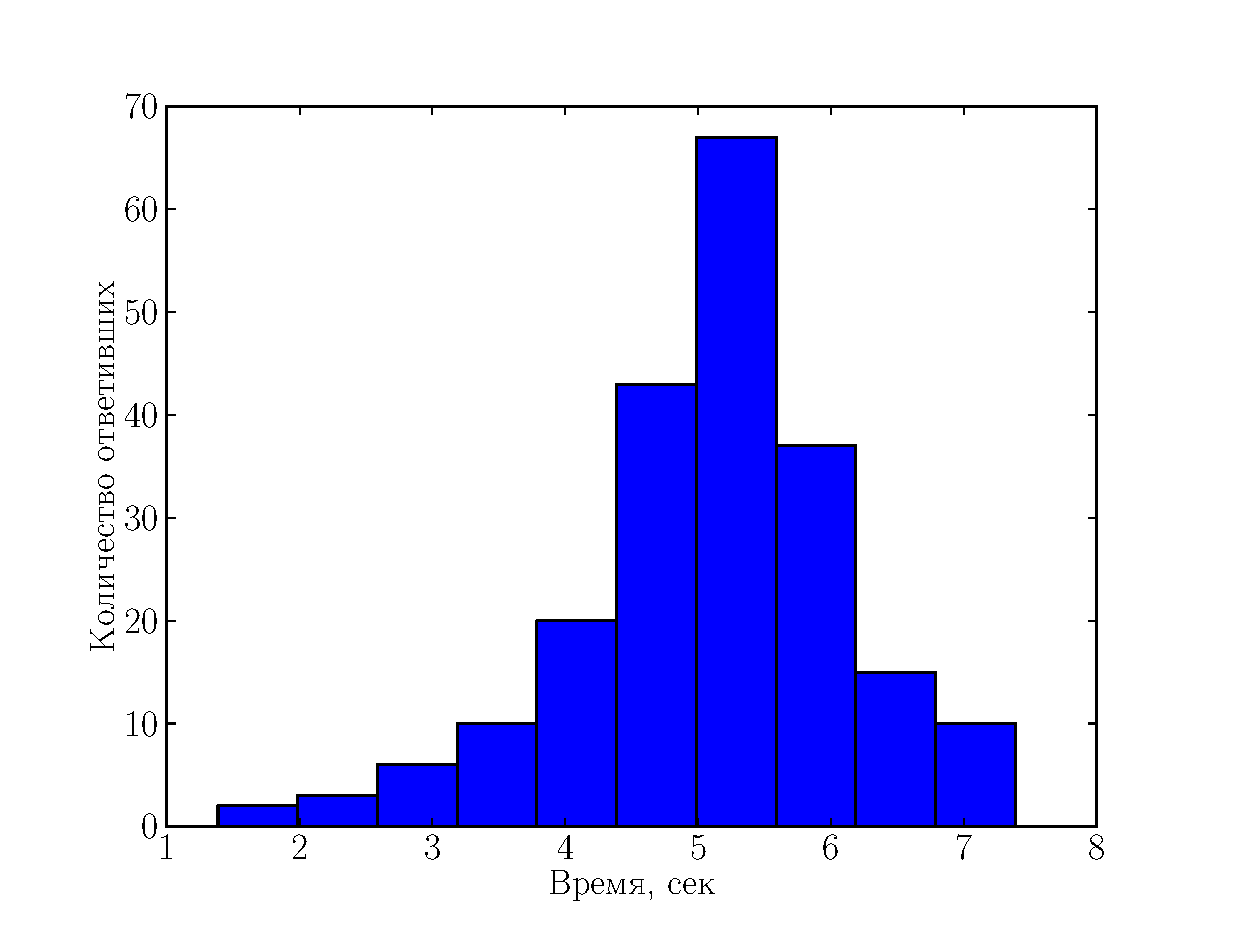
\includegraphics[scale=0.6]{test1.eps}
\caption{Гистограмма времени ответа (логарифмический масштаб)}
\end{figure}

Как видно из данного примера, прменение логарифмического преобразования к выборке по времени ответа обучающихся на конкретную задачу в системе дистанционного обучения позволяет получить симметричный вид распределения, который походит на гауссовское распределение. Проверка на гауссовость приводится в следующем пункте.

\subsection{Проверка предположения о гауссовости}

Проверим гипотезу о гауссовом распределении времени ответа студента. Для этого сформулируем основную и альтернативную гипотезы следующего вида:
$$
\begin{array}{lll}
H_0 &:& t_{ij} \sim N\left(\mu,\sigma^2\right)\\
H_1 &:& t_{ij} \mbox{ имеет другое распределение}
\end{array}
$$

\subsection{Оценка параметров модели по выборке}
\label{opmpv}

Проведём оценку параметров модели согласно пункту \ref{opm}.

\subsection{Применение модели к реальным данным}

Использя данные оценки, полученные в пункте \ref{opmpv}, продемонстрируем работу модели для выявления отклонений в поведении студентов.